\documentclass{standalone}

\usepackage[OT1]{fontenc}
\renewcommand*\familydefault{\sfdefault}
\usepackage{helvet,sfmath}
\usepackage{siunitx}

\usepackage{tikz}
\usetikzlibrary{arrows,calc,patterns}
\usepackage{tikz,tkz-euclide}


\definecolor{BlueDefault}{rgb}{0.2,0.2,0.7}

\begin{document}

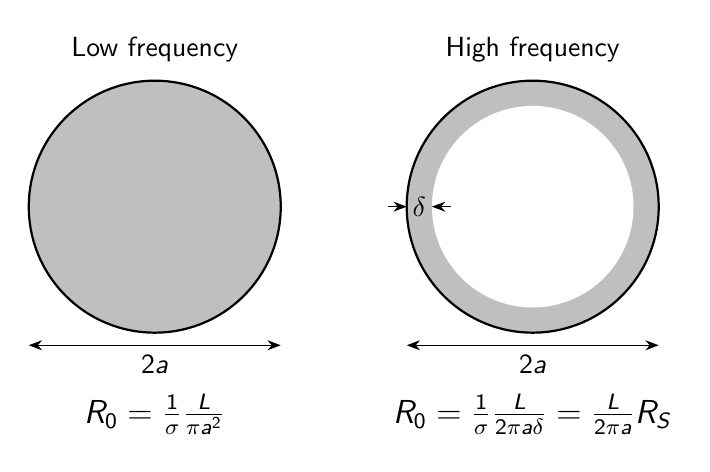
\begin{tikzpicture}[scale=0.8]
    \draw[fill=lightgray, thick] (-3,0) circle (2);
    \draw[thick, fill=lightgray] (3,0) circle (2);
    \draw[draw=none, fill=white] (3,0) circle (1.6);
    \draw
    (3,2.5) node{High frequency}
    (-3,2.5) node{Low frequency}
    ;
    \draw[-Stealth] (0.7,0) to (1,0);
    \draw[-Stealth] (1.7,0) to (1.4,0);
    \draw (1.2,0) node{\(\delta\)};

    \draw[Stealth-Stealth] (-5,-2.2) to (-1,-2.2);
    \draw[Stealth-Stealth] (5,-2.2) to (1,-2.2);
    \draw
    (-3,-2.5) node{\(2a\)}
    (3,-2.5) node{\(2a\)}
    ;
    \draw
    (-3,-3.3) node{\large \(R_0 = \frac{1}{\sigma} \frac{L}{\pi a^2}\)}
    (3,-3.3) node{\large \(R_0 = \frac{1}{\sigma} \frac{L}{2 \pi a \delta} = \frac{L}{2 \pi a} R_S\)}
    ;
\end{tikzpicture}    

\end{document}